\documentclass[../../main.tex]{subfiles}

\begin{document}

\begin{figure}[H]
    \centering
    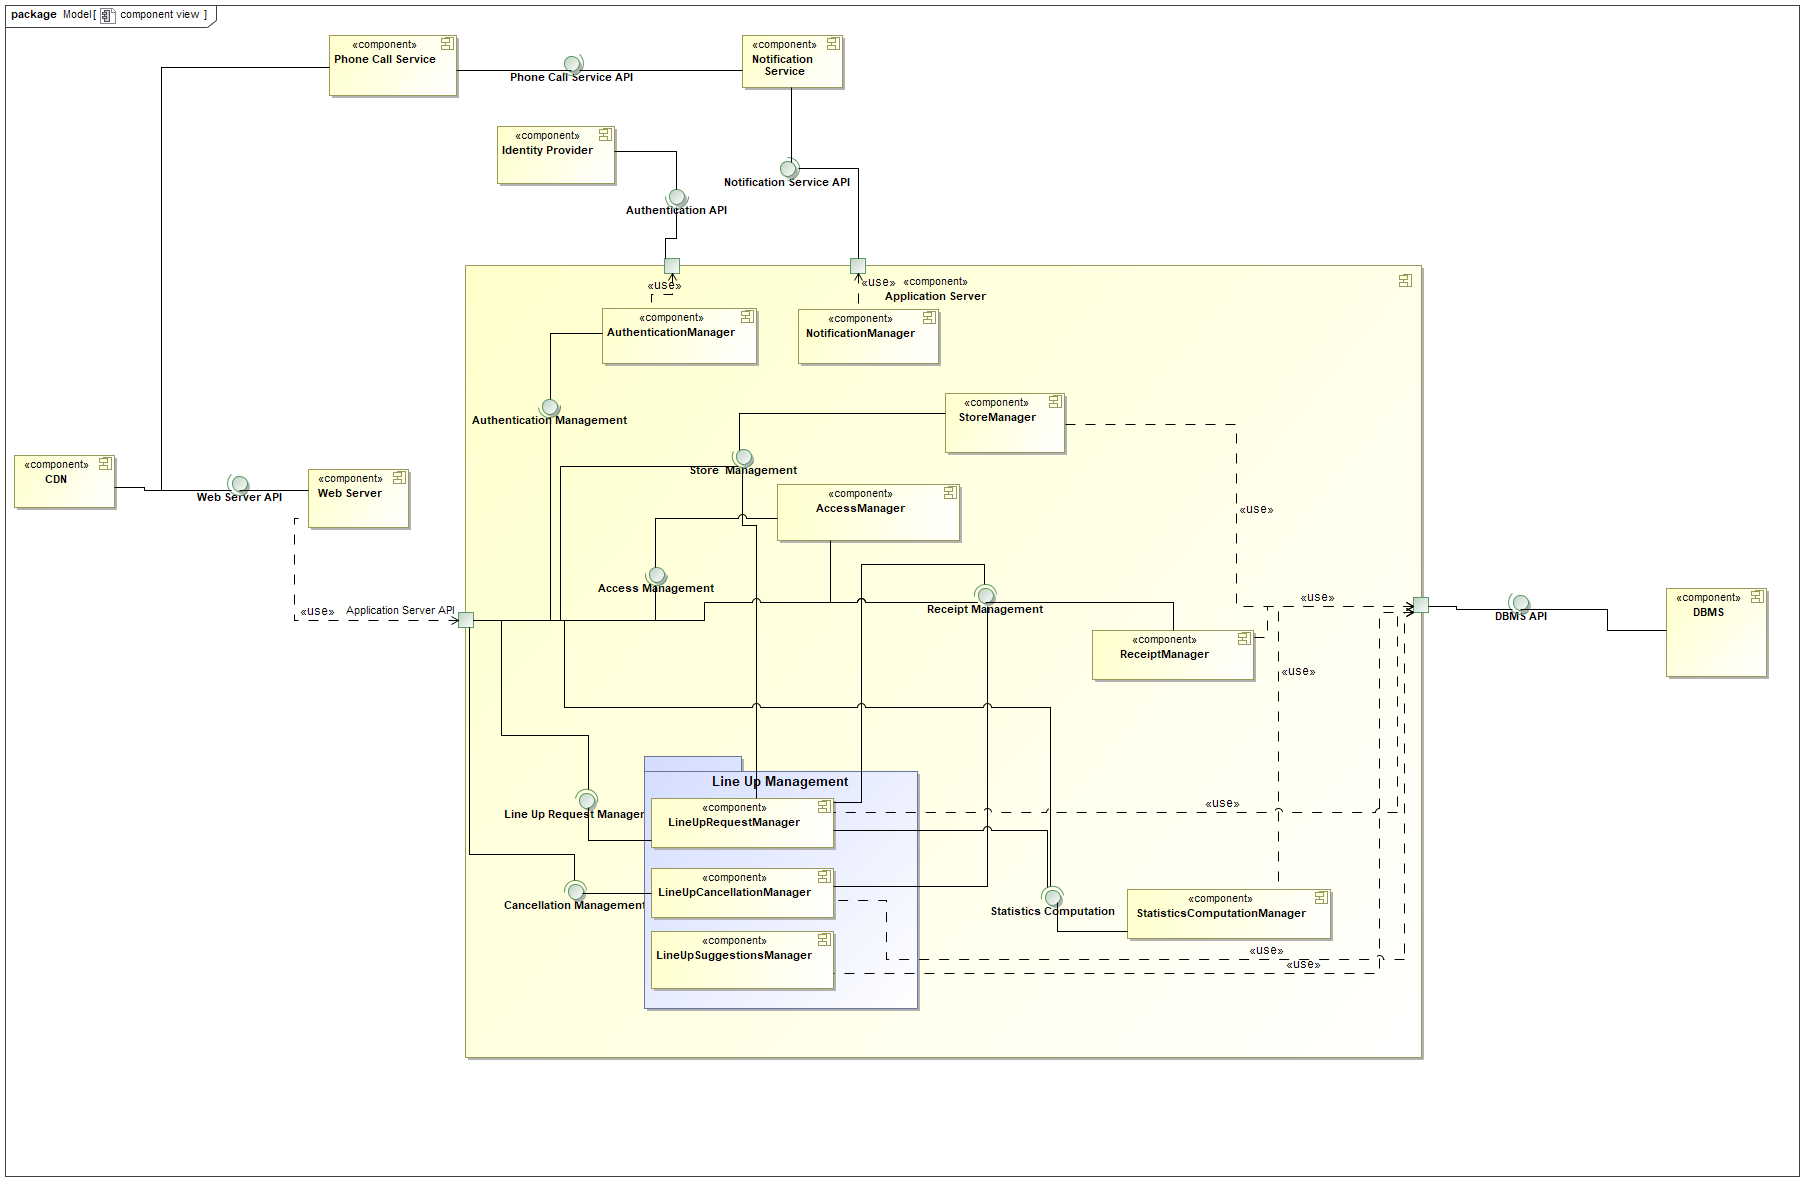
\includegraphics[width=\textwidth]{component_view.png}
    \caption{
        Component diagram
    }
\end{figure}

The component diagram above presents a general view of the application. 
The image describes the application server and its components with the highest level of detail, 
as developers will have to implement the business logic themselves. The other nodes in the system, as well as the services, 
are depicted more abstractly. Developers of the project might choose to use commercial off the shelf solutions 
to provide those APIs, thus losing control on the internal components, but accelerating the development.

\end{document}
